\documentclass{report}
\usepackage{graphicx, tikz-cd, float, titlepic, booktabs} % Required for inserting images
\usepackage{pgfplots}
\pgfplotsset{compat=1.15}
\usepackage{mathrsfs}
\usetikzlibrary{arrows}
\usepackage{amsmath, amssymb, amsthm, amsfonts, siunitx, physics, gensymb}
\AtBeginDocument{\RenewCommandCopy\qty\SI}
\usepackage[version=4]{mhchem}
\usepackage[most,many,breakable]{tcolorbox}
\usepackage{xcolor, fancyhdr, varwidth}
\usepackage[Glenn]{fncychap}
%Options: Sonny, Lenny, Glenn, Conny, Rejne, Bjarne, Bjornstrup
\usepackage{hyperref, cleveref}
\usepackage{icomma, enumitem} %comma as decimal and continue enumerate with [resume]
\usepackage{plimsoll} %use standard state symbol with \stst
\usepackage[danish]{babel}
%%%%%%%%%%%%%%%%%%%%%%%%%%%%%%
% SELF MADE COLORS
%%%%%%%%%%%%%%%%%%%%%%%%%%%%%%
\definecolor{myg}{RGB}{56, 140, 70}
\definecolor{myb}{RGB}{45, 111, 177}
\definecolor{myr}{RGB}{199, 68, 64}
\definecolor{mytheorembg}{HTML}{F2F2F9}
\definecolor{mytheoremfr}{HTML}{00007B}
\definecolor{mylenmabg}{HTML}{FFFAF8}
\definecolor{mylenmafr}{HTML}{983b0f}
\definecolor{mypropbg}{HTML}{f2fbfc}
\definecolor{mypropfr}{HTML}{191971}
\definecolor{myexamplebg}{HTML}{F2FBF8}
\definecolor{myexamplefr}{HTML}{88D6D1}
\definecolor{myexampleti}{HTML}{2A7F7F}
\definecolor{mydefinitbg}{HTML}{E5E5FF}
\definecolor{mydefinitfr}{HTML}{3F3FA3}
\definecolor{notesgreen}{RGB}{0,162,0}
\definecolor{myp}{RGB}{197, 92, 212}
\definecolor{mygr}{HTML}{2C3338}
\definecolor{myred}{RGB}{127,0,0}
\definecolor{myyellow}{RGB}{169,121,69}
\definecolor{myexercisebg}{HTML}{F2FBF8}
\definecolor{myexercisefg}{HTML}{88D6D1}
%%%%%%%%%%%%%%%%%%%%%%%%%%%%%%%%%%%%%%%%%%%%%%%%%%%%%%%%%%%%%%%%%%%%%%
% Box environments for theorems and problems
%%%%%%%%%%%%%%%%%%%%%%%%%%%%%%%%%%%%%%%%%%%%%%%%%%%%%%%%%%%%%%%%%%%%%
\setlength{\parindent}{1cm}
%================================
% Question BOX
%================================
\makeatletter
\newtcbtheorem{question}{Opgave}{enhanced,
	breakable,
	colback=white,
	colframe=myb!80!black,
	attach boxed title to top left={yshift*=-\tcboxedtitleheight},
	fonttitle=\bfseries,
	title={#2},
	boxed title size=title,
	boxed title style={%
			sharp corners,
			rounded corners=northwest,
			colback=tcbcolframe,
			boxrule=0pt,
		},
	underlay boxed title={%
			\path[fill=tcbcolframe] (title.south west)--(title.south east)
			to[out=0, in=180] ([xshift=5mm]title.east)--
			(title.center-|frame.east)
			[rounded corners=\kvtcb@arc] |-
			(frame.north) -| cycle;
		},
	#1
}{def}
\makeatother
%================================
% DEFINITION BOX
%================================

\newtcbtheorem[]{Definition}{Definition}{enhanced,
	before skip=2mm,after skip=2mm, colback=red!5,colframe=red!80!black,boxrule=0.5mm,
	attach boxed title to top left={xshift=1cm,yshift*=1mm-\tcboxedtitleheight}, varwidth boxed title*=-3cm,
	boxed title style={frame code={
					\path[fill=tcbcolback]
					([yshift=-1mm,xshift=-1mm]frame.north west)
					arc[start angle=0,end angle=180,radius=1mm]
					([yshift=-1mm,xshift=1mm]frame.north east)
					arc[start angle=180,end angle=0,radius=1mm];
					\path[left color=tcbcolback!60!black,right color=tcbcolback!60!black,
						middle color=tcbcolback!80!black]
					([xshift=-2mm]frame.north west) -- ([xshift=2mm]frame.north east)
					[rounded corners=1mm]-- ([xshift=1mm,yshift=-1mm]frame.north east)
					-- (frame.south east) -- (frame.south west)
					-- ([xshift=-1mm,yshift=-1mm]frame.north west)
					[sharp corners]-- cycle;
				},interior engine=empty,
		},
	fonttitle=\bfseries,
	title={#2},#1}{def}
\newtcbtheorem[]{definition}{Definition}{enhanced,
	before skip=2mm,after skip=2mm, colback=red!5,colframe=red!80!black,boxrule=0.5mm,
	attach boxed title to top left={xshift=1cm,yshift*=1mm-\tcboxedtitleheight}, varwidth boxed title*=-3cm,
	boxed title style={frame code={
					\path[fill=tcbcolback]
					([yshift=-1mm,xshift=-1mm]frame.north west)
					arc[start angle=0,end angle=180,radius=1mm]
					([yshift=-1mm,xshift=1mm]frame.north east)
					arc[start angle=180,end angle=0,radius=1mm];
					\path[left color=tcbcolback!60!black,right color=tcbcolback!60!black,
						middle color=tcbcolback!80!black]
					([xshift=-2mm]frame.north west) -- ([xshift=2mm]frame.north east)
					[rounded corners=1mm]-- ([xshift=1mm,yshift=-1mm]frame.north east)
					-- (frame.south east) -- (frame.south west)
					-- ([xshift=-1mm,yshift=-1mm]frame.north west)
					[sharp corners]-- cycle;
				},interior engine=empty,
		},
	fonttitle=\bfseries,
	title={#2},#1}{def}

\newtcbtheorem{theo}%
    {Theorem}{}{theorem}
\newtcolorbox{prob}[1]{colback=red!5!white,colframe=red!50!black,fonttitle=\bfseries,title={#1}}
%================================
% NOTE BOX
%================================

\usetikzlibrary{arrows,calc,shadows.blur}
\tcbuselibrary{skins}
\newtcolorbox{note}[1][]{%
	enhanced jigsaw,
	colback=gray!20!white,%
	colframe=gray!80!black,
	size=small,
	boxrule=1pt,
	title=\textbf{Note:},
	halign title=flush center,
	coltitle=black,
	breakable,
	drop shadow=black!50!white,
	attach boxed title to top left={xshift=1cm,yshift=-\tcboxedtitleheight/2,yshifttext=-\tcboxedtitleheight/2},
	minipage boxed title=1.5cm,
	boxed title style={%
			colback=white,
			size=fbox,
			boxrule=1pt,
			boxsep=2pt,
			underlay={%
					\coordinate (dotA) at ($(interior.west) + (-0.5pt,0)$);
					\coordinate (dotB) at ($(interior.east) + (0.5pt,0)$);
					\begin{scope}
						\clip (interior.north west) rectangle ([xshift=3ex]interior.east);
						\filldraw [white, blur shadow={shadow opacity=60, shadow yshift=-.75ex}, rounded corners=2pt] (interior.north west) rectangle (interior.south east);
					\end{scope}
					\begin{scope}[gray!80!black]
						\fill (dotA) circle (2pt);
						\fill (dotB) circle (2pt);
					\end{scope}
				},
		},
	#1,
}
%================================
% EXAMPLE BOX
%================================
\newtcbtheorem[number within=section]{Example}{Example}
{%
	colback = myexamplebg
	,breakable
	,colframe = myexamplefr
	,coltitle = myexampleti
	,boxrule = 1pt
	,sharp corners
	,detach title
	,before upper=\tcbtitle\par\smallskip
	,fonttitle = \bfseries
	,description font = \mdseries
	,separator sign none
	,description delimiters parenthesis
}
{ex}
%================================
% THEOREM BOX
%================================

\tcbuselibrary{theorems,skins,hooks}
\newtcbtheorem[number within=section]{Theorem}{Theorem}
{%
	enhanced,
	breakable,
	colback = mytheorembg,
	frame hidden,
	boxrule = 0sp,
	borderline west = {2pt}{0pt}{mytheoremfr},
	sharp corners,
	detach title,
	before upper = \tcbtitle\par\smallskip,
	coltitle = mytheoremfr,
	fonttitle = \bfseries\sffamily,
	description font = \mdseries,
	separator sign none,
	segmentation style={solid, mytheoremfr},
}
{th}

%%%%%%%%%%%%%%%%%%%%%%%%%%%%%%%%%%%%%%%%%%%%%%%%%%%%%%%%%%%%%%%%%
% SELF MADE COMMANDS
%%%%%%%%%%%%%%%%%%%%%%%%%%%%%%
\newcommand{\sol}{\setlength{\parindent}{0cm}\textbf{\textit{Løsning:}}\setlength{\parindent}{1cm}}
%%%%%%%%%%%%%%%%%%%%%%%%%%%%%%%%%
\usepackage[tmargin=2cm,rmargin=1in,lmargin=1in,margin=0.85in,bmargin=2cm,footskip=.2in]{geometry}\pagestyle{fancy}
\lhead{Minrui Kevin Zhou 3.b}
\rhead{H7}

\title{H7\\
{\Large \textbf{3.b Fysik A}}}
\author{Kevin Zhou}
\date{\today}

\begin{document}
\maketitle
\begin{note}
  Databog Fysik Kemi (2007) er anvendt ved beregningerne.
\end{note}
\begin{question}{Kølefryseskab}{}
I et amerikansk kølefryseskab løsnes isterninger ved hjælp af et elektrisk varmelegeme. Strømstyrken gennem varmelegemet er 1,40 A. Varmelegemet omsætter elektrisk energi med effekten 168 W.
\begin{itemize}
  \item[a.] Bestem spændingsfaldet over varmelegemet.
\end{itemize}
Isterningerne fryses i en form, som er lavet af aluminium. Formens masse er 0,544 kg.
Når isterningerne skal løsnes, tændes varmelegemet i 90 s.
Herved opvarmes formen fra -18 °C til 0 °C, og desuden smeltes noget af isen.
\begin{itemize}
  \item[b.] Vurdér massen af is, der smeltes, når isterningerne skal løsnes.
\end{itemize}
\end{question}
\sol \\
\textbf{a.}
Der gælder, at effekten i en komponent er produktet af spændingsfaldet over den og strømstyrken gennem den:
\begin{equation*}
\begin{split}
  P=U \cdot I \iff U=\frac{P}{I}
\end{split}
\end{equation*}
Vi udregner nu $U$.
\begin{equation*}
\begin{split}
  U&=\frac{P}{I}\\
  &=\frac{168 \;\unit{W} }{1,40 \;\unit{A} }\\
  &=120 \;\unit{V} 
\end{split}
\end{equation*}
Altså er spændingsfaldet over varmelegemet $120 \;\unit{V} $. \\[1ex]
\textbf{b.}
Vi antager, at det kun er isen, der smeltes, som varmes op, og resten af isen forbliver den samme temperatur.
Da det både er den is, der smeltes og aluminiumsformen, der opvarmes, så må varmeenergien, der tilføres være 
\begin{equation*}
\begin{split}
  E&=E _{\text{opvarmning} } + E _{\text{smeltning} }\\
  &=\left(m _{\text{is} } \cdot c _{\text{is} } + m _{\text{alu} } \cdot c _{\text{alu} }\right) \cdot \Delta T + m _{\text{is} } \cdot L_s(\text{is})\\
  &=m _{\text{is} } \cdot \left(c _{\text{is} } \cdot \Delta T + L_s(\text{is} )\right) + m _{\text{alu} } \cdot c _{\text{alu} }\cdot \Delta T
\end{split}
\end{equation*}
hvor $c _{x}$ er den specifikke varmekapacitet af stoffet $x$, $L_s(\text{is} )$ er den specifikke smeltevarme for is og $m _{\text{is} }$ er massen af den is, som smeltes. 
Da effekten $P$ blot er energi per tid, så må der gælde
\begin{equation*}
\begin{split}
  P=\frac{E}{t} &\iff E=P \cdot t \\
  &\iff m _{\text{is} } \cdot \left(c _{\text{is} } \cdot \Delta T + L_s(\text{is} )\right) + m _{\text{alu} } \cdot c _{\text{alu} }\cdot \Delta T=P \cdot t\\
  &\iff m _{\text{is} } \cdot \left(c _{\text{is} } \cdot \Delta T + L_s(\text{is} )\right) =P \cdot t- m _{\text{alu} } \cdot c _{\text{alu} }\cdot \Delta T\\
  &\iff m _{\text{is} }=\frac{P \cdot t- m _{\text{alu} } \cdot c _{\text{alu} }\cdot \Delta T}{c _{\text{is} } \cdot \Delta T + L_s(\text{is} )}
\end{split}
\end{equation*}
Vi kan nu udregne massen af isen, der smeltes.
\begin{equation*}
\begin{split}
  m _{\text{is} }&=\frac{P \cdot t- m _{\text{alu} } \cdot c _{\text{alu} }\cdot \Delta T}{c _{\text{is} } \cdot \Delta T + L_s(\text{is} )}\\
  &=\frac{168 \;\unit{W} \cdot 90 \;\unit{s} - 0,544 \;\unit{kg}  \cdot 900 \;\unit{\frac{J}{kg \cdot \celsius}} \cdot 18 \;\unit{\celsius}}{2040 \;\unit{\frac{J}{kg \cdot \celsius}}  \cdot 18 \;\unit{\celsius}  + 334,4 \cdot 10^3 \;\unit{J/kg} }\\
  &\approx 0,017 \;\unit{kg} \\
  &=17 \;\unit{g} 
\end{split}
\end{equation*}
Altså smeltes $17 \;\unit{g} $ is når isterningerne skal løsnes. 
\begin{question}{Tinisotopen \ce{^100Sn} }{}
Ved et eksperiment er det lykkedes forskere at fremstille 250 kerner af isotopen \ce{^100Sn}. Isotopen \ce{^100Sn} er radioaktiv med halveringstiden 1,18 s.
\begin{itemize}
  \item[a.] Vurdér, hvor lang tid der går, inden der kun er 20 kerner tilbage af isotopen \ce{^100Sn}.
\end{itemize}
Isotopen \ce{^100Sn} henfalder ved et $\beta ^+$-henfald. 
\begin{itemize}
  \item[b.] Opskriv reaktionsskemaet for henfaldet af \ce{^100Sn}. 
  \item[c.] Benyt masserne af de indgående partikler til at bestemme henfaldets Q-værdi. 
\end{itemize}
\end{question}
\sol \\
\textbf{a.}
Fra henfaldsloven har vi, at 
\begin{equation*}
\begin{split}
  N=N_0 \cdot \left(\frac{1}{2}\right) ^{\frac{t}{T _{\frac{1}{2}}}} &\iff \frac{t}{T _{\frac{1}{2}}}=\log_{\frac{1}{2}}\left(\frac{N}{N_0}\right) \\
  &\iff t=T _{\frac{1}{2}} \cdot \log_{\frac{1}{2}}\left(\frac{N}{N_0}\right)
\end{split}
\end{equation*}
hvor $N$ er antallet af kerner til tiden $t$, og $N_0$ er antallet kerner til tiden $t=0$. 
Vi kan nu udregne tiden.
\begin{equation*}
\begin{split}
  t&=T _{\frac{1}{2}} \cdot \log_{\frac{1}{2}}\left(\frac{N}{N_0}\right)\\
  &=1,18 \;\unit{s} \cdot \log_{\frac{1}{2}}\left(\frac{20}{250}\right) \\
  &\approx 4,30 \;\unit{s} 
\end{split}
\end{equation*}
Der går altså $4,30 \;\unit{s} $, inden der kun er 20 kerner af \ce{^100Sn} tilbage. \\[1ex]
\textbf{b.}
Ved et $\beta ^+$-henfald udsender kernen en positron og en elektronneutrino.
Reaktionsskemaet bliver 
\[
\ce{_50^100Sn -> ^100_49In + ^0_1e + \nu_e} 
\] 
For god ordens skyld, bekræfter vi, at nukleontallet $A$, ladningen $Z$ og leptontallet $L$ er bevarede:
\begin{equation*}
\begin{split}
  A&=100=100\\
  Z&=50=49+1\\
  L&=0=0-1+1
\end{split}
\end{equation*}
\textbf{c.}
Vi beregner henfaldets $Q$-værdi, hvor masserne er slået op på Ptable.com.
\begin{equation*}
\begin{split}
  Q&=-\Delta m \cdot c^2\\
  &=\left( m\left(\ce{_50^100Sn} \right) - m\left(\ce{^100_49In} \right)- m \left(^0_1e\right) \right) \cdot c^2\\
  &=\left(99.939044343 \;\unit{u} - 99.931110851 \;\unit{u} - 0,000548580 \;\unit{u} \right) \cdot 931,49 \;\unit{MeV/u} \\
  &\approx 6,8790 \;\unit{MeV} 
\end{split}
\end{equation*}
Henfaldets Q-værdi er altså $6,8790 \;\unit{MeV} $.
\begin{question}{Supernovaen XT 110621}{}
  Supernovaen XT 110621 blev opdaget ved observationer af en kraftig udsendelse af stråling fra en fjern galakse. Supernovaen udsendte røntgenstråling med energien $2,8 \cdot 10^{39}$ J i løbet af 315 s.
\begin{itemize}
  \item[a.] Bestem med hvilken gennemsnitlig effekt, supernovaen udsendte røntgenstråling.
\end{itemize}
Afstanden til den galakse, hvor supernovaeksplosionen fandt sted, blev bestemt ud fra galaksens spektrum, som er vist på figuren. Spektrallinjen med den største intensitet har laboratoriebølgelængden 656,3 nm. 
\begin{itemize}
  \item[b.] Vurdér galaksens nuværende fart væk fra os.
\end{itemize}
\end{question}
\sol \\
\textbf{a.}
Vi beregner den gennemsnitlige effekt, der blot er energi per tid.
\begin{equation*}
\begin{split}
  P&=\frac{E}{t}\\
  &=\frac{2,8 \cdot 10 ^{39} \;\unit{J} }{315 \;\unit{s} }\\
  &\approx 8,9 \cdot 10 ^{36} \;\unit{W}
\end{split}
\end{equation*}
Den gennemsnitlige effekt, hvormed supernovaen udsendte røntgenstråling er altså $8,9 \cdot 10 ^{36} \;\unit{W} $.\\[1ex]
\textbf{b.}
Vi aflæser på spektret, at spektrallinjen med den største intensitet har den observerede bølgelængde $\lambda _{\text{obs} }=718 \;\unit{nm} $ (se \cref{fig:spek}).
\begin{figure}[H]
\begin{center}
  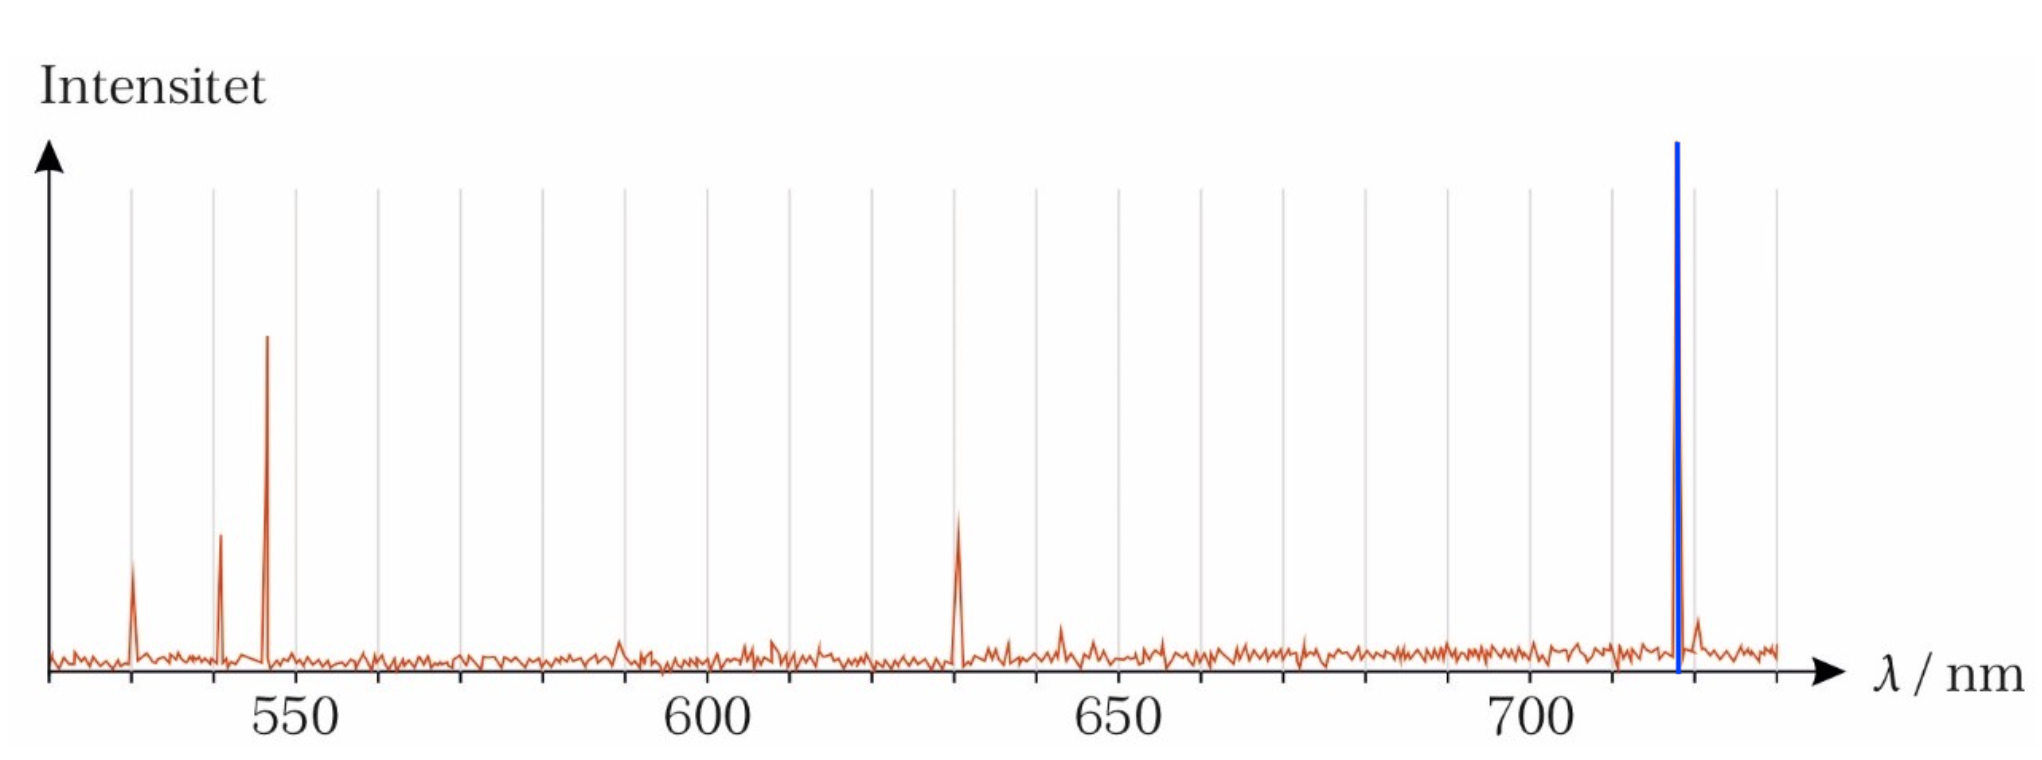
\includegraphics[width=\textwidth]{spek.png}
\end{center}
\caption{Aflæsning på spektret}
\label{fig:spek}
\end{figure}
Vi kan nu udregne galaksens nuværende fart væk fra os.
\begin{equation*}
\begin{split}
  v_0&=c \cdot \frac{\lambda _{\text{obs} }- \lambda _{\text{lab}}}{\lambda _{\text{lab} }}\\
  &=3,00 \cdot 10 ^{5} \;\unit{km/s} \cdot \frac{718 \;\unit{nm} - 656,3 \;\unit{nm} }{656,3 \;\unit{nm} }\\
  &\approx 2,82 \cdot 10^4 \;\unit{km/s} 
\end{split}
\end{equation*}
Galaksens nuværende fart væk fra os er altså $2,82 \cdot 10^4 \;\unit{km/s} $.
\begin{question}{Løbebånd}{}
En person løber 10 km på et løbebånd med farten 12 km/h.
\begin{itemize}
  \item[a.] Hvor lang tid tager det personen at løbe 10 km på løbebåndet?
\end{itemize}
Bilaget Løbebånd er en video, som viser en mindre del af tidsrummet, hvor et løbebånd er ved at stoppe, fordi løbebåndets nødstop er aktiveret. Der er 1,0 m mellem de to gule streger. Løbebåndet bremser med konstant acceleration.

Mens en person løber på løbebåndet med farten 12 km/h, bliver nødstoppet aktiveret.
\begin{itemize}
  \item[b.] Brug bilaget Løbebånd til at bestemme, hvor langt personen skal løbe på løbebåndet, inden det er stoppet helt.
\end{itemize}
\end{question}
\sol \\
\textbf{a.}
Vi finder et udtryk for tiden
\begin{equation*}
\begin{split}
  v=\frac{s}{t} \iff  t=\frac{s}{v}
\end{split}
\end{equation*}
Vi kan nu udregne tiden.
\begin{equation*}
\begin{split}
  t&=\frac{s}{v}\\
  &=\frac{10 \;\unit{km} }{12 \;\unit{km/h} }\\
  &=\frac{5}{6} \;\unit{h} \cdot 60 \;\unit{min/h} \\
  &\approx 50 \;\unit{min} 
\end{split}
\end{equation*}
Det tager altså 50 minutter at løbe 10 km på løbebåndet. \\[1ex]
\textbf{b.}
En videotracking af sted ift. tid af det blå bånd på løbebåndet laves i Logger Pro, hvilket ses i \cref{fig:video}.
\begin{figure}[H]
\begin{center}
  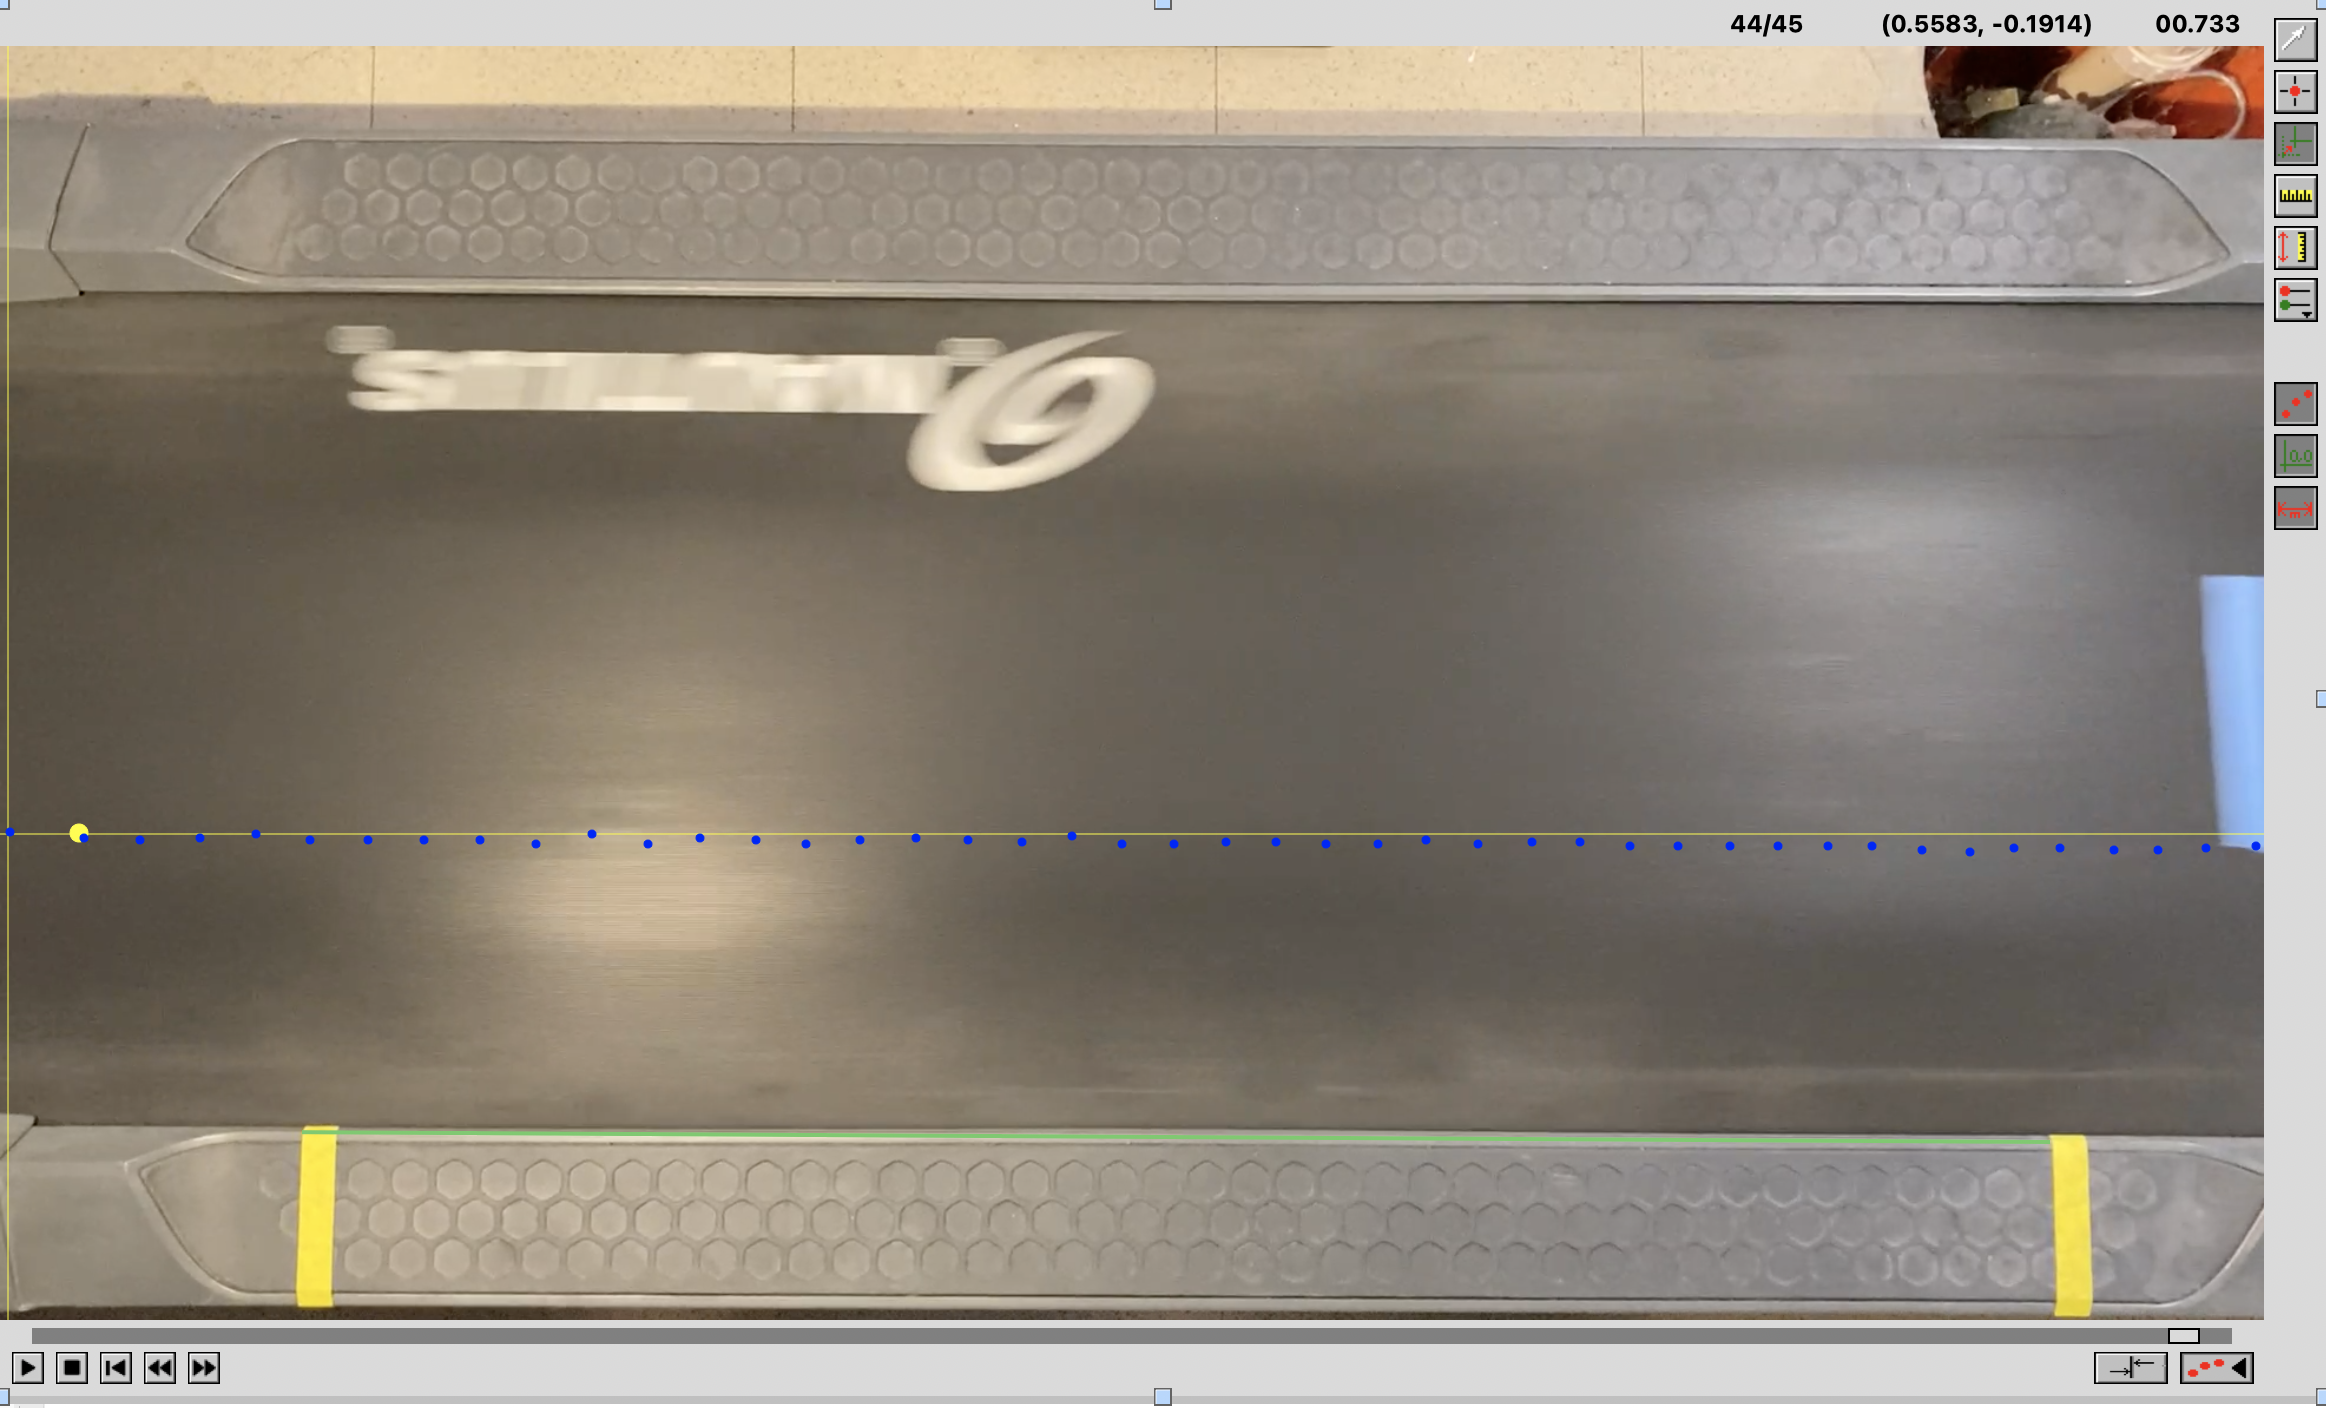
\includegraphics[width=\textwidth]{video.png}
\end{center}
\caption{Videotracking i Logger Pro}
\label{fig:video}
\end{figure}
Siden løbebåndet bremser med konstant acceleration, så laves en lineær regression på punkterne på $(t,v_x)$-grafen, hvilket ses i \cref{fig:tv}.
Det ses, at punkterne ligger tilnærmelsesvist på en ret linje.
\begin{figure}[H]
\begin{center}
  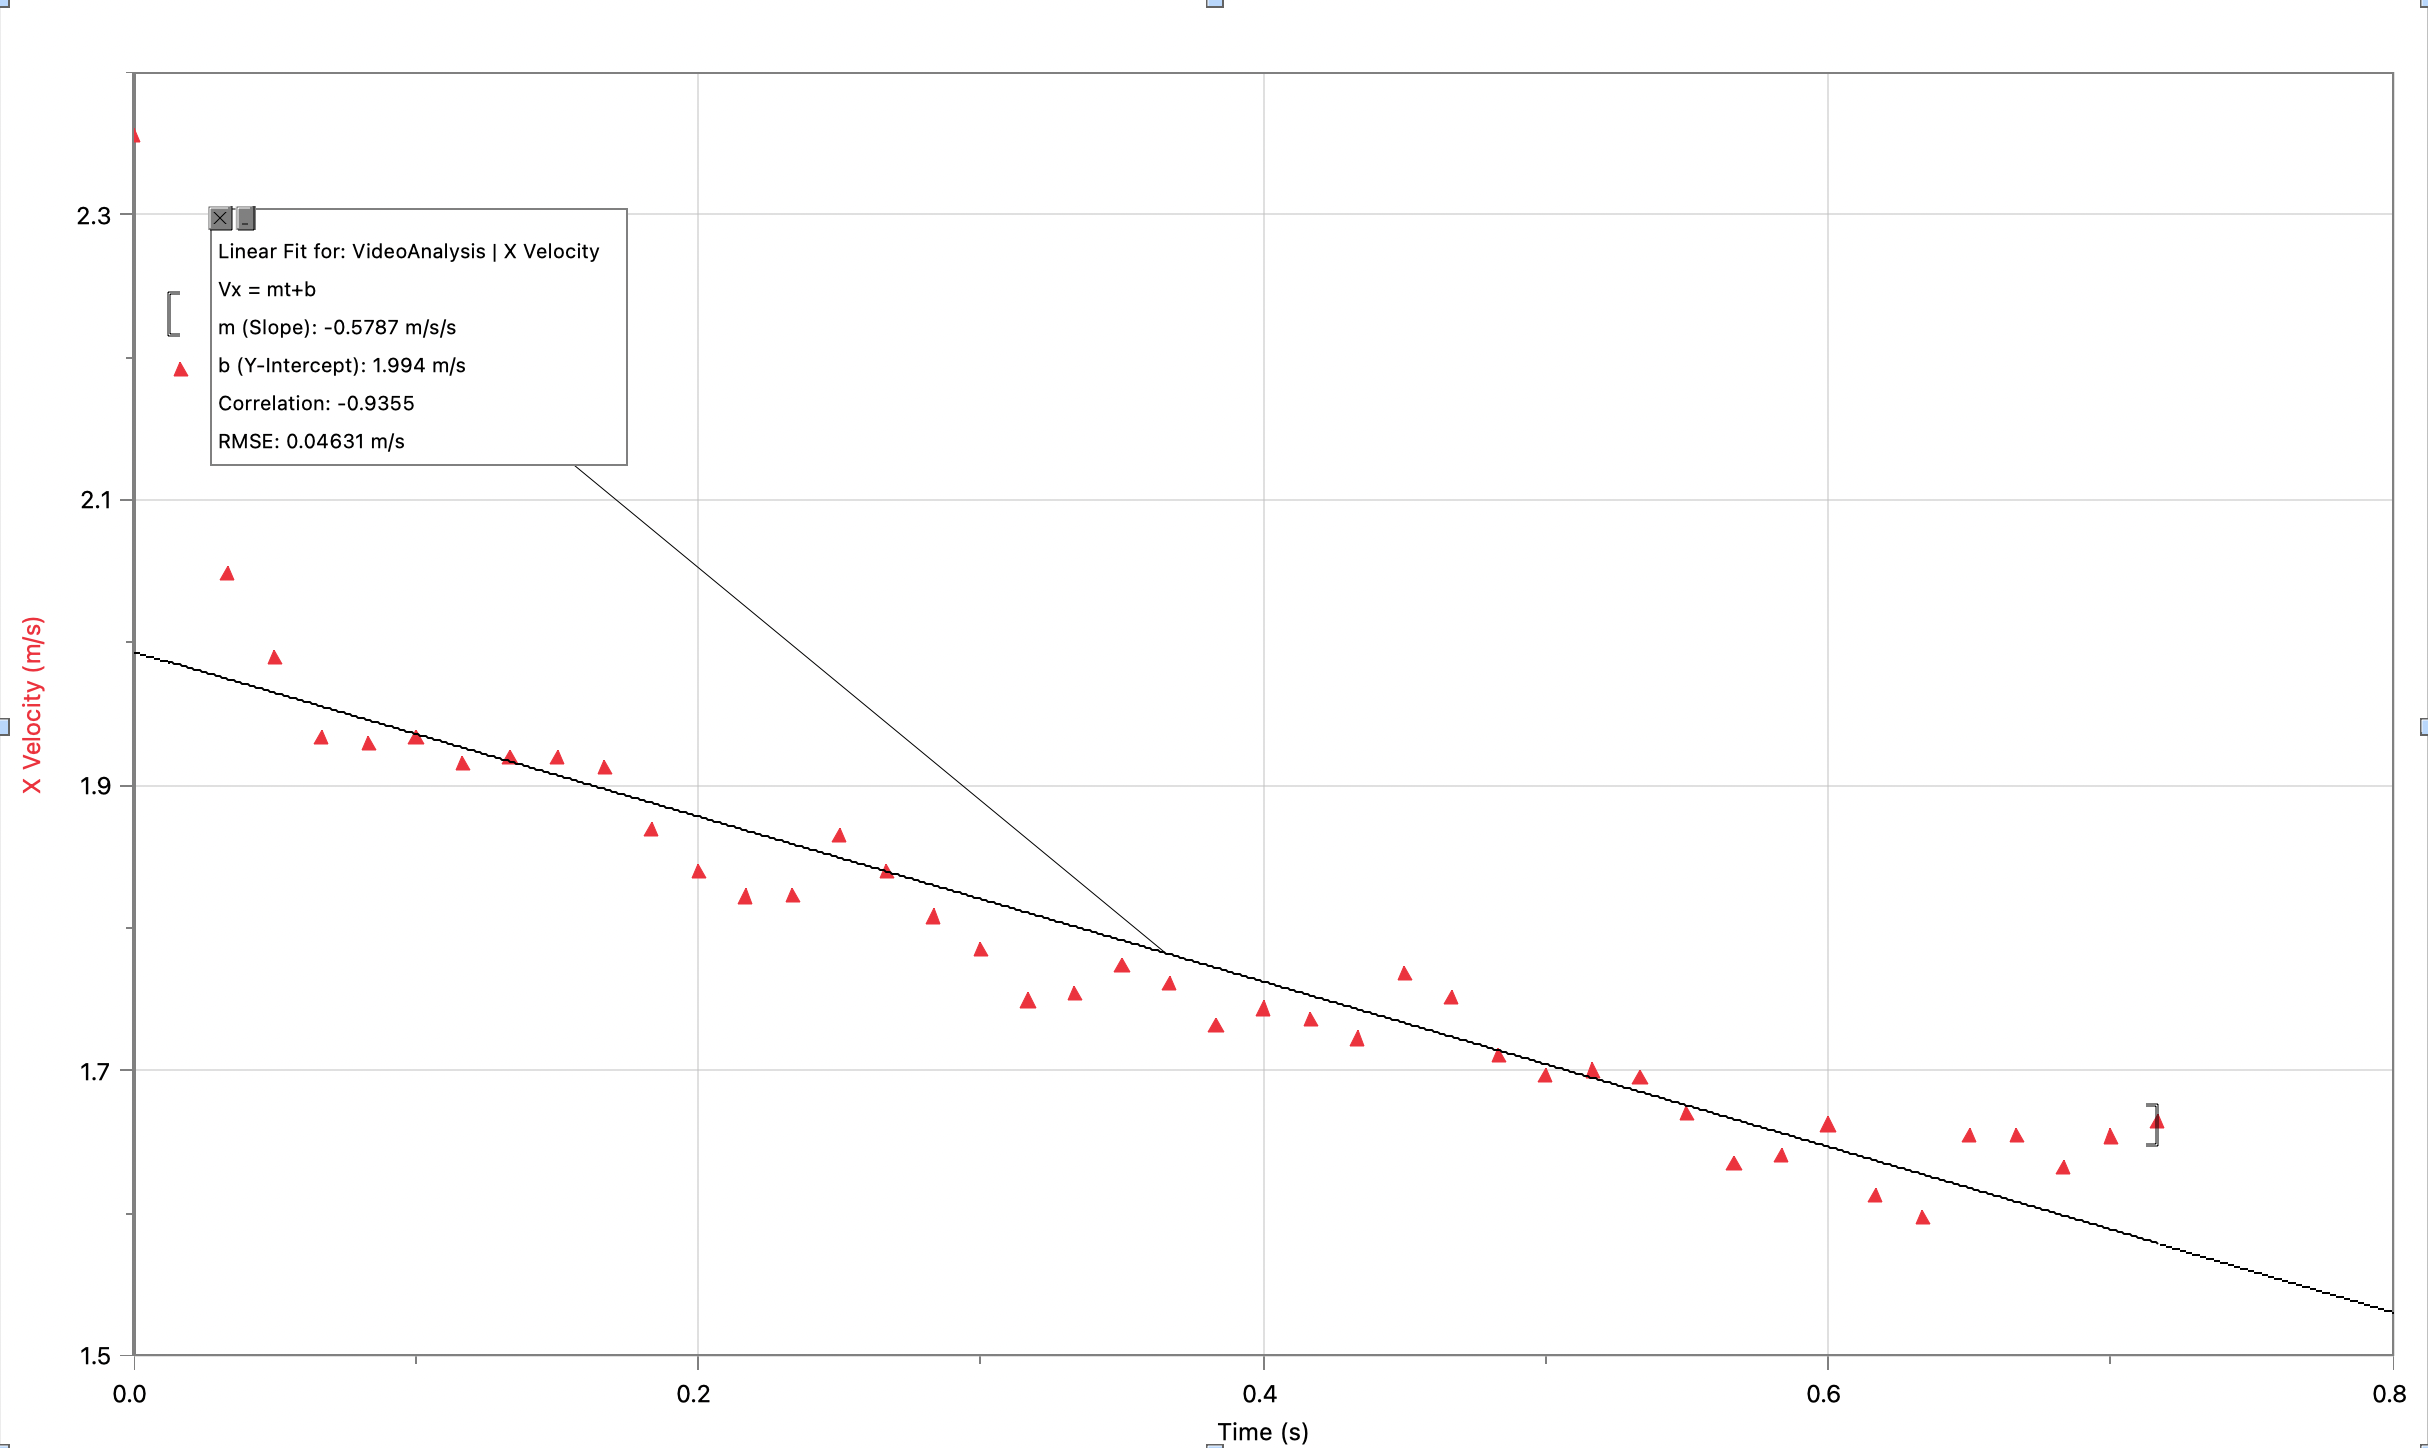
\includegraphics[width=\textwidth]{tv.png}
\end{center}
  \caption{Lineær regression på $(t,v_x)$-grafen i Logger Pro}
\label{fig:tv}
\end{figure}
Det ses, at punkterne ligger tilnærmelsesvist på den rette linje, og vi har fra regressionen, at accelerationen i $x$-retningen er
\begin{equation*}
\begin{split}
  a=-0,5787 \;\unit{m/s^2}  
\end{split}
\end{equation*}
Vi kan nu udregne bremselængden til båndet er helt stoppet.
\begin{equation*}
\begin{split}
  \Delta s &=\frac{v_2^2-v_1^2}{2 \cdot a}\\
  &=\frac{\left(0 \;\unit{m/s} \right)^2 - \left(\frac{12}{3,6}\;\unit{m/s} \right)^2}{2 \cdot (-0,5787 \;\unit{m/s^2}) }\\
  &\approx 2,9 \;\unit{m} 
\end{split}
\end{equation*}
Altså skal personen $2,9 \;\unit{m} $ på løbebåndet inden den stopper helt. 




\end{document}
